
\chapter{Materials and Methods}

\section{Instruments and Apparatus}

The experiment described requires a number of computer systems and associated
hardware to run the simulation and capture appropriate data. This equipment is
described in the following chapter.

\begin{enumerate}
  \item Hub/Managed Router

  Most modern network appliances used for routing, even those labelled as hubs,
  include switching capabilities, which means that packets routed are only
  delivered to the addressed host. This makes eavesdropping difficult. For
  the purpose of this experiment a Netgear DS106 dual speed hub was used. A hub
  does not examine packet delivery information, it simple broadcasts all packets
  received to every connected port, allowing for passive eavesdropping without
  complicated network configuration \parencite{website:hub-reference}.

  \item 'tcpdump' Software

  The tcpdump software captures network packets that are transferred using
  network interfaces attached to the current hardware \parencite{:2009cr}.  It is
  available on most operating systems and supports a flexible filtering language
  for capturing only the specific packets desired. The format of output produced
  by tcpdump is well documented \parencite{:nx} which makes it ideal for
  transformation and processing by third party tools. Tcpdump version 4.0.0
  combined with libpcap 1.0.0 was used for this experiment.

  \item Tor Software

  The Tor software is available on a number of operating systems and the Tor
  project makes packages available for the Ubuntu operating system.

  \item Weka Software

  Weka is data mining software which includes tools for classification of data
  sources using a wide variety of machine learning algorithms
  \parencite{Hall:2009p7662,Bouckaert:2010we}. It supports processing of an
  input Attribute-Relation File Format (ARFF), a file which contains ASCII text
  describing a list of items with common attributes known as instances.
  Instances can be given an attribute which provides a nominal classification
  for verification purposes in Weka. Version 3.6.4 of Weka was used for
  classification during this experiment.

  \item netAI Software

  netAI is capable of processing packet traces such as the one produced by
  tcpdump, analysing flows and producing ARFF files containing every flow
  identified as an individual instance \parencite{swinbut:2006fk}. Each instance
  includes many attributes produced from statistical analysis of these flows
  which are useful for traffic classification. An explanation of the statistics
  gathered by netAI is included in table \ref{table:netmate-attributes}.

  \item VirtualBox Software

  VirtualBox software allows multiple guest operating systems to run in an
  isolated virtual environment on a host operating system \parencite{:fk}.
  It is free software and supports both snapshots and a remote control facility
  which make it useful for running a controlled experiment \parencite{Oracle:2011kx}.
  VirtualBox version 3.2.6 r63112 was used in this experiment.

  \item Ruby Software

  Ruby is an object orientated, dynamic programming language which is useful for
  rapid prototyping and is supported by a large community that has developed
  powerful add on software in the form of Ruby Gems \parencite{:2010uq}. These
  Gems include support for the Selenium browser testing framework, process
  monitoring, dynamic web content generation and automated testing. The Ruby
  1.8.7 (2010-01-10 patchlevel 249) Ubuntu package was installed where Ruby was
  required. The exact version of all gems used in the experiment are shown in
  table \ref{table:gems}.

  \begin{center}
    \begin{minipage}[t]{\linewidth}
      \begin{table}[H]
        \begin{tabular}{llr}
          \toprule
          Gem name & Purpose & Version \\
          \midrule
          bundler & Application gem manager & 1.0.2 \\
          daemon\_controller & Monitor and control daemon processes & 0.2.6 \\
          rspec & Testing and control of selenium & 1.3.0 \\
          selenium-client & Control browser using selenium and ruby & 1.2.18 \\
          haml & A simple HTML like markup language & 3.0.21 \\
          rack & Rack web serving framework & 1.2.1 \\
          sinatra & Ruby web framework & 1.0 \\
          \bottomrule
        \end{tabular}
        \caption{Ruby Gems}
        \label{table:gems}
      \end{table}
    \end{minipage}
  \end{center}

  \item Ubuntu Linux Software

  The Ubuntu Linux operating system is freely available Linux operating system
  available for desktop personal computers \parencite{:2010ly}. It comes
  packaged with the 'tcpdump' software and can be configured in a reliable and
  consistent way with typical set of POSIX tools and the 'apt-get' package
  manager \parencite{Pereira:2011uq}. Both the desktop and server editions were
  used for this experiment, version 10.04 commonly referred to as lucid lynx.

  \item Selenium Software

  Selenium is a web testing framework which allows automated testing of web pages
  through any Javascript enabled web browser \parencite{:2010ys}. A web browser
  can be controlled remotely using the Selenium Remote Control Server component,
  which in turn can be controlled with a number of programming languages including
  Ruby. Using Selenium the typical interactions a user makes when viewing a
  website can be simulated. Selenium version 1.0.6 was used for this experiment.

  \item Firefox Software

  Firefox is a web browser developed by the Mozilla organization and freely
  available for most desktop personal computers \parencite{Foundation:2011fk}.
  It's strong standards compliance \parencite{Hammond:2010fk} and popularity
  \parencite{:2010kx,:2010vn} on the simulation platform make it an ideal
  candidate for this experiment. The Ubuntu Firefox package was used in this
  expriment, version 3.6.8.

  \item OpenSSH Software

  OpenSSH is a freely available suite of connectivity tools
  \parencite{:2010zr,:ve} that supports remote command execution
  \parencite{Tucker:2010ly}. The client component of OpenSSH is installed by
  default on the Ubuntu operating system and the server component is easily
  installed using the apt-get package management system. The version used for
  this experiment was OpenSSH\_5.3p1 Debian-3ubuntu4, OpenSSL 0.9.8k 25 Mar 2009.

  \item Apache Software

  The Apache web server is the most prevalent web server used on the Internet
  \parencite{2010:dq}. The Apache web server can serve static web content over
  both the HTTP and HTTPS protocols \parencite{Foundation:2011uq}. Combined with
  software such as Sinatra it can serve dynamic web content. Apache version
  2.2.14/Ubuntu was used to serve web sites in this experiment.

  \item Sinatra Software

  Sinatra is a simple framework for creating dynamic web applications using the
  Ruby programming language \parencite{:2010bh}. Sinatra requires very little
  configuration and development time to develop dynamic web applications.
  Sinatra version 1.0 was used in this experiment.

  \item RSpec

  RSpec is a behaviour driven testing framework for Ruby which allows the
  creation of examples in an easy to read Domain Specific Language (DSL)
  \parencite{Chelimsky:2010vn}. It is well integrated with Selenium which makes
  it ideal for running large suites of Selenium tests. RSpec version 1.3.0 was
  used in this experiment.

\end{enumerate}

\section{Procedure}

The experiment involves two stages, an initial configuration stage to prepare
equipment, install software, configure and test the design and the final stage
of executing the simulation to capture packet traces.

The simulation involves three separate phases of equal length, each simulating a
different kind of network traffic:

\begin{enumerate*}
  \item Web requests over HTTPS
  \item Web requests over HTTP proxied by Tor
  \item Web requests over HTTPS proxied by Tor
\end{enumerate*}

\subsection{Hardware Configuration}

Four identical desktop computer systems were prepared and arranged as shown
in figure \ref{fig:physical-setup}.

\begin{figure}[H]
  \centering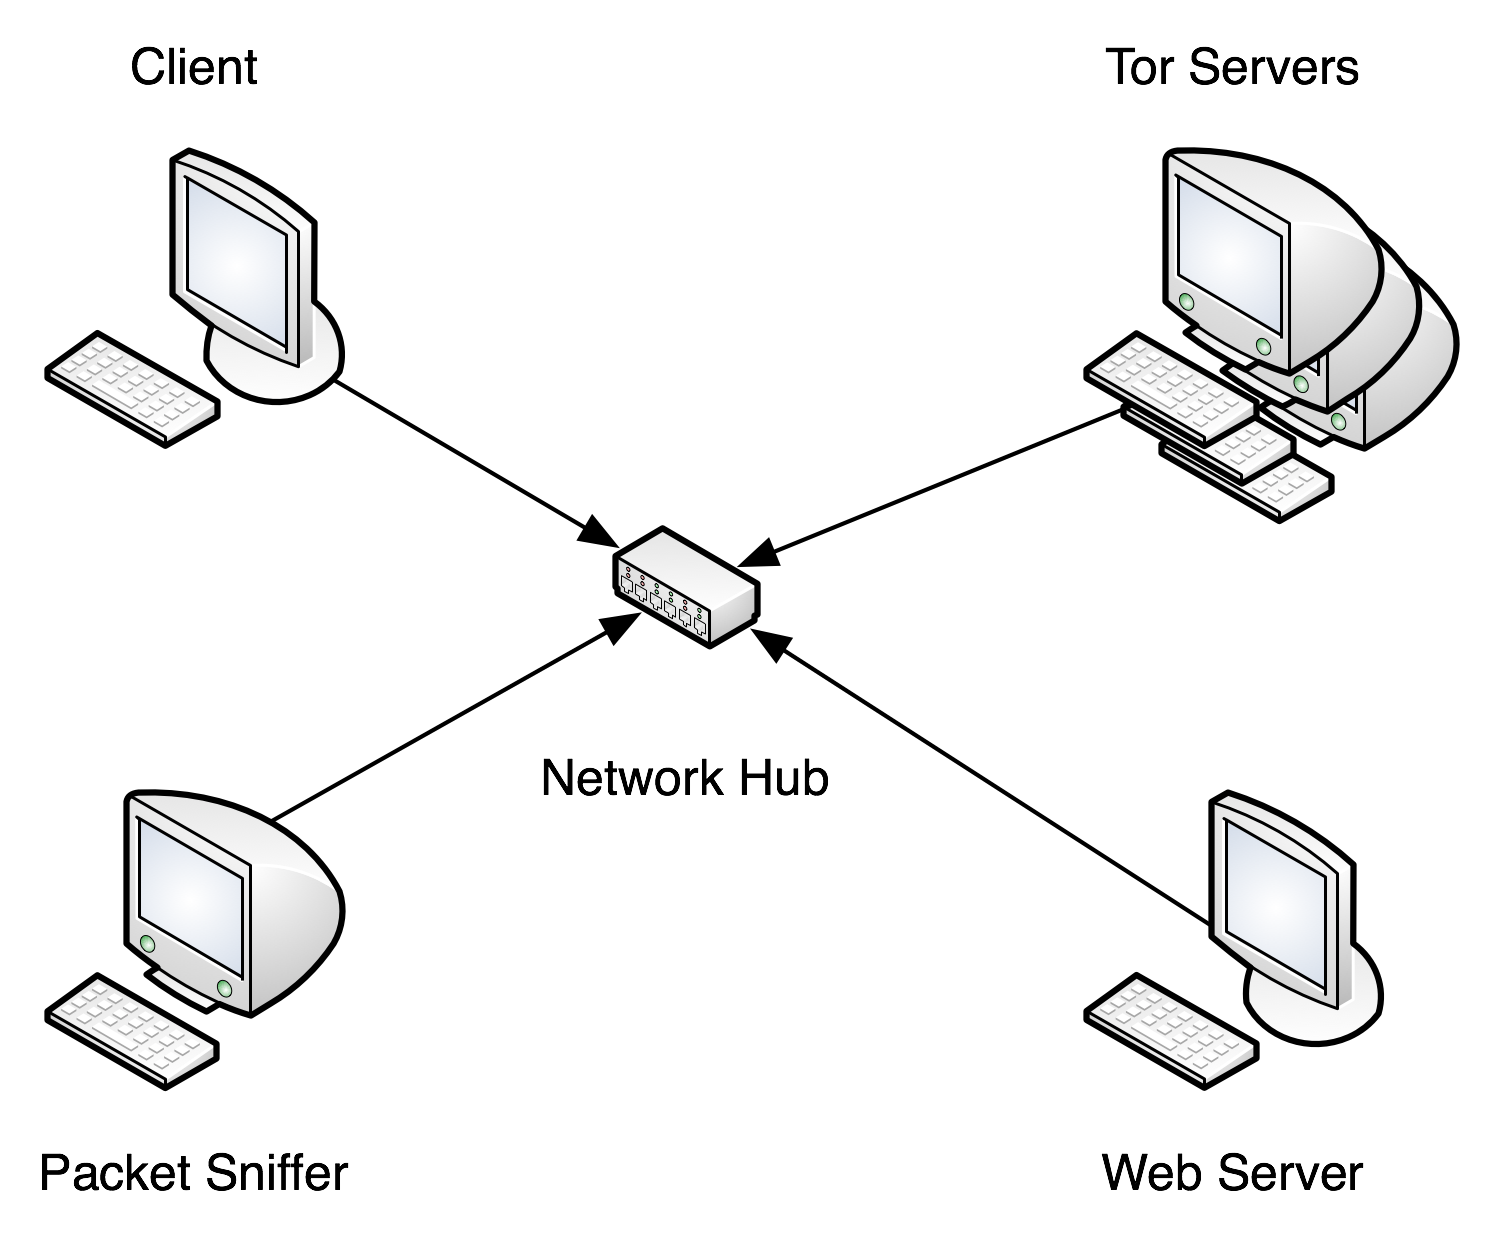
\includegraphics[scale=0.7]{physical-setup}
  \caption{Physical Setup}
  \label{fig:physical-setup}
\end{figure}

\subsection{Software Configuration}

Table \ref{table:hosts} shows the role, edition of the Ubuntu operating system
installed and the IP address assigned to each host in the experiment network.

\begin{table}[H]
  \begin{tabular}{lrr}
    \toprule
    Role & Operating System Version & IP Address\\
    \midrule
    Client Host & Desktop & 192.168.0.100\\
    Server Host & Desktop & 192.168.0.101\\
    Tor Host & Desktop & 192.168.0.102\\
    \midrule
    Sniffing System & Server & 192.168.0.200\\
    \midrule
    Client Guest & Desktop & 192.168.0.16\\
    Server Guest & Server & 192.168.0.17\\
    Tor Network Guest & Server & 192.168.0.18\\
    \bottomrule
  \end{tabular}
  \caption{System Roles}
  \label{table:hosts}
\end{table}

Figure \ref{fig:network-diagram} shows the placement of applications and relevant
data flows when running the simulation in HTTPS mode.

\begin{figure}[H]
  \centering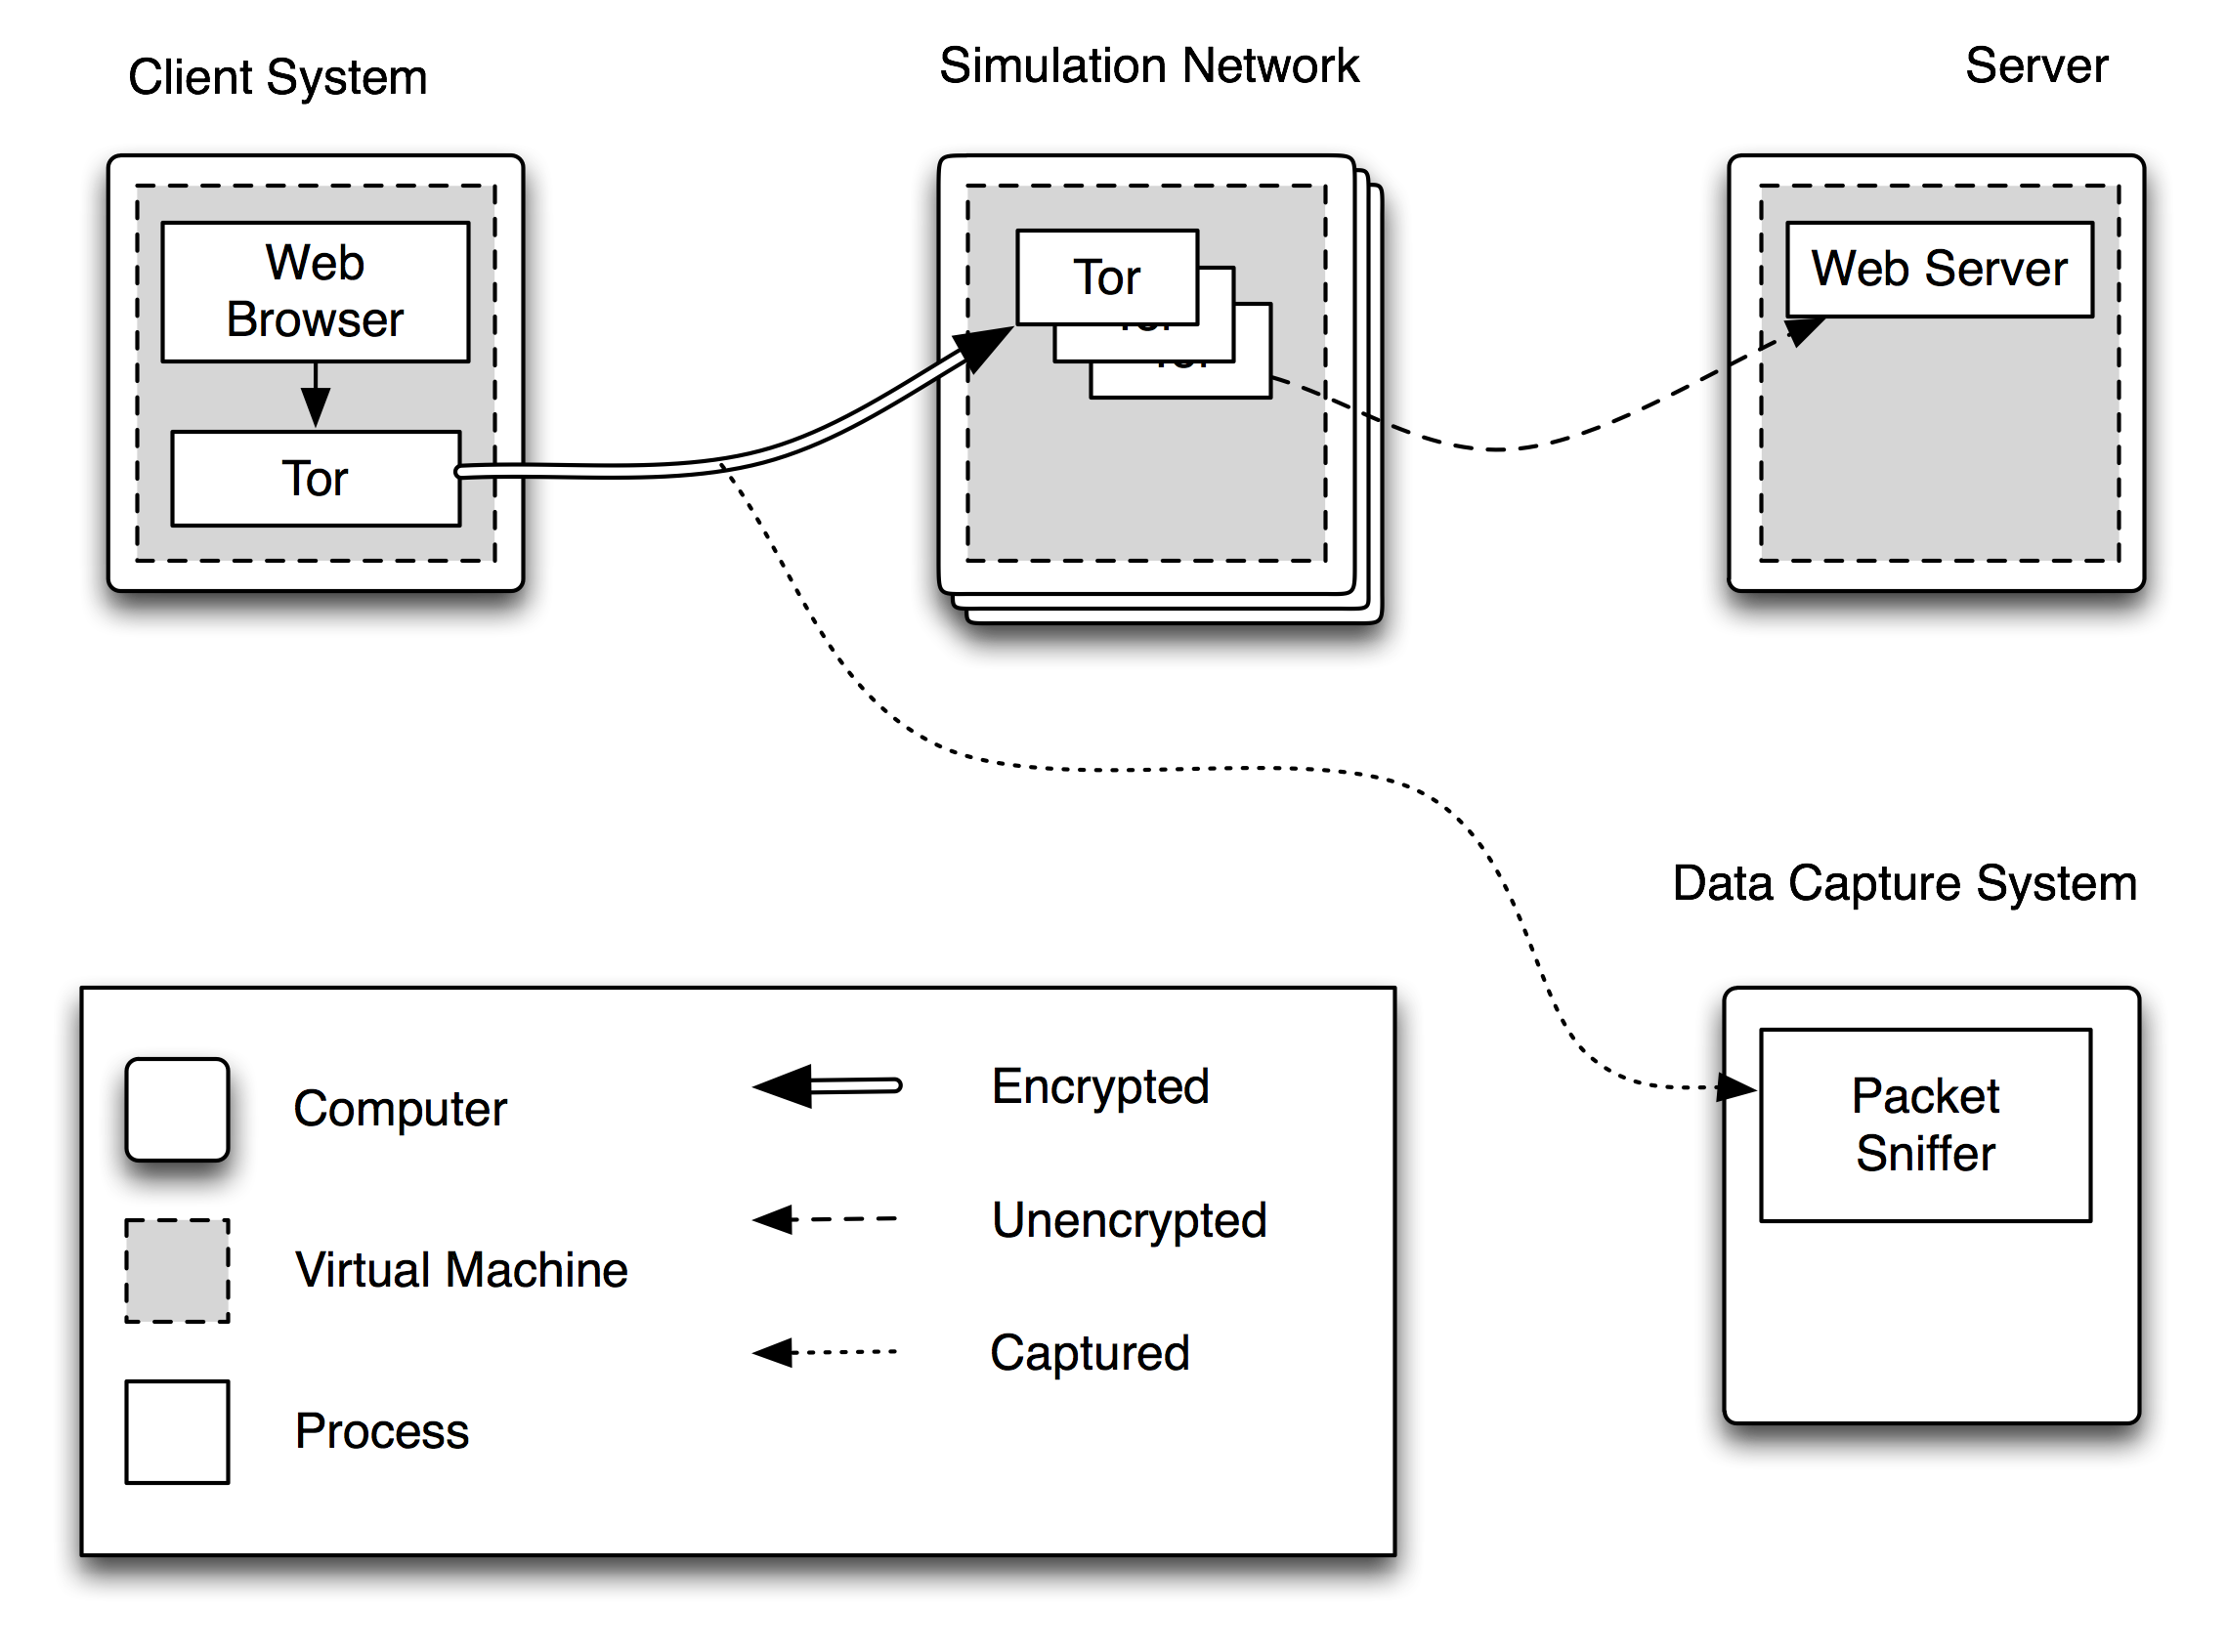
\includegraphics[width=\linewidth]{network-diagram}
  \caption{Network Diagram: Phase 1}
  \label{fig:network-diagram}
\end{figure}

Figure \ref{fig:network-diagram-with-tor} shows the network configuration when
running the experiment in HTTP over Tor mode.

\begin{figure}[H]
  \centering\includegraphics[width=\linewidth]{network-diagram-with-tor}
  \caption{Network Diagram: Phase 2}
  \label{fig:network-diagram-with-tor}
\end{figure}

Figure \ref{fig:network-diagram-with-tor-encrypted} shows the network configuration when
running the experiment in HTTPS over Tor mode.

\begin{figure}[H]
  \centering\includegraphics[width=\linewidth]{network-diagram-with-tor-encrypted}
  \caption{Network Diagram: Phase 3}
  \label{fig:network-diagram-with-tor-encrypted}
\end{figure}

\subsection{Standard OS Installation Procedure}
\label{section:os_install}

All systems in the experiment use a variation of the Ubuntu Linux operating
system. Table \ref{table:config-options} specifies the options supplied when
installing each operating system for the experiment.

\begin{table}[H]
  \begin{tabular}{lr}
    \toprule
    Prompt & Value\\
    \midrule
    Where are you? & Australia/Perth\\
    Which layout is most similar to your keyboard? & USA\\
    How do you want to partition the disk? & Erase and use the entire disk\\
    What is your name? & John Barker\\
    What name do you want to use to log in? & john\\
    \bottomrule
  \end{tabular}
  \caption{Ubuntu Installation Parameters}
  \label{table:config-options}
\end{table}

Each system is given a statically assigned IP address, this is done by editing
the file \verb+/etc/network/interfaces+ and changing the line
\verb+iface eth0 inet dhcp+ to:

\begin{lstlisting}[language=sh]
iface eth0 inet static
  address 192.168.0.16
  netmask 255.255.255.0
  network 192.168.0.0
  broadcast 192.168.0.255
\end{lstlisting}

Substituting \verb+eth0+ with the physical network interface identifier as
appropriate, and the address \verb+192.168.0.16+ with the desired value. All
systems were assigned IP Addresses as listed in \ref{table:hosts}.

\subsection{Sniffing System}

The sniffing system is prepared as described in \ref{section:os_install} with an
Ubuntu 10.04 server CD. The base install of Ubuntu server has all the required
packages included so no additional software installation is required.

An init.d script was created to execute the tcpdump program with a specific
filter string after the system had powered on. All capture files were limited to
1MB in size and put into a time stamped directory. To ensure that only relevant
packets were collected the filter string was tuned for each phase of the
experiment. The filter string for each phase is shown below.

Phase 1:
\begin{lstlisting}[language=sh]
tcp port 443
\end{lstlisting}

Phase 2 and 3:
\begin{lstlisting}[language=sh]
tcp portrange 5000-5015
\end{lstlisting}

The capture script appears below with the filter string as required for phase 2
and 3:

\begin{lstlisting}[language=sh]
#!/bin/bash
export capture_date=`date`
cd /home/john/ssl-captures
mkdir "./${capture_date}"
tcpdump -vv -C 1 -i eth0 -w "./${capture_date}/capture.dat" tcp portrange 5001-5015
\end{lstlisting}

\subsection{Host Systems}

The host systems all run an identically configured Ubuntu 10.04 desktop
operating system, except for the IP address which is configured as described in
\ref{table:hosts}. To support the guest operating systems, VirtualBox is
required. The procedure used to install VirtualBox is described below:

\begin{enumerate*}
  \item Edit the file \verb+/etc/apt/sources.lst+ and add the line:
\begin{lstlisting}[language=sh]
deb http://download.virtualbox.org/virtualbox/debian lucid non-free
\end{lstlisting}
  \item Install the GPG key for the Virtual Box packages:
\begin{lstlisting}[language=sh]
wget -q http://download.virtualbox.org/virtualbox/debian/oracle_vbox.asc -O- | sudo apt-key add -
\end{lstlisting}
  \item Then install VirtualBox 3.2 with the command:
\begin{lstlisting}[language=sh]
sudo apt-get update && sudo apt-get install virtualbox-3.2
\end{lstlisting}
\end{enumerate*}

The guest operating systems were copied across using a USB thumb drive and
installed using the VirtualBox import feature.

\subsubsection{Client Host}

One of the host systems was set aside as a management system, which is
responsible for ensuring the experiment runs and restarts it if there are any
problems.

For delivering remote commands from the management system to other hosts without
interactive prompts, SSH is used with automatic private key authentication. To
enable automatic private key authentication, first a private key was generated
by executing the following commands in a terminal prompt:

\begin{enumerate*}
  \item \verb+ssh-keygen+
  \item Press enter to use default keyfile (\verb+/Users/john/.ssh/id_rsa+)
  \item Press enter twice to supply a blank passphrase
\end{enumerate*}

The public key is then copied to the other hosts using secure copy (SCP), for example:
\begin{lstlisting}[language=sh]
  scp ~/.ssh/id_rsa.pub john@192.168.0.101:
\end{lstlisting}

This file was then appended to the authorized hosts file on each system, by
executing the following command from each host system:
\begin{lstlisting}[language=sh]
  cat id_rsa.pub >> ~/.ssh/authorized_keys
\end{lstlisting}

The management script runs on the management system to monitor experiment
progress. This simple script manages the VirtualBox instances on the other hosts
by remotely executing VirtualBox control commands using SSH. It ensures that
each time the experiment is finished, the VirtualBox instances are rolled back
and restarted. If the experiment takes too long, it is manually restarted. The
script listens on a port for a connection from the experiment client which
indicates the experiment has finished. Figure \ref{manager-flow-diagram}
contains a diagram which outlines the basic flow of the manager script.

\begin{figure}[H]
  \centering\includegraphics[scale=0.7]{manager-flow}
  \caption{Manager Script Flow Chart}
  \label{manager-flow-diagram}
\end{figure}

Note that restarting each snapshot ensures that the system clock of each guest
operating system is synchronized with that of the host operating system. The
Tor network is sensitive to differences in time between hosts and this ensures
correct operation.

\subsection{Guest Systems}

\subsubsection{Client Guest}

The client system runs Ubuntu 10.04 Desktop Operating System as well as a
number of applications that allow it to perform automated web browsing. Tor is
configured on this system but disabled for the first phase of the simulation.

The software installed on this system includes:

\begin{itemize*}
  \item Ruby
  \item Rubygems:
    \begin{itemize*}
      \item Selenium
      \item DaemonController
      \item RSpec
    \end{itemize*}
  \item Selenium-RC
  \item Firefox web browser
  \item Tor
\end{itemize*}

The client operation is controlled by a Ruby script which ensures that the
Selenium-RC server is running, executes a number of Selenium browser simulations
using RSpec and reports completion by connecting to an open socket on the
management system. This script is configured to run at boot time so that as soon
as the system is powered on the simulation commences. The complete client script
is included in the Appendix, section \ref{client-script}.

The simulation component consists of 170 different RSpec examples which emulate
various profiles of website traffic against 30 different example websites
provided by the Server system.

\paragraph{Tor}
\label{install-tor}

Tor is installed on the client guest using the following procedure:

\begin{enumerate*}
  \item Edit the file \verb+/etc/apt/sources.lst+ and add the line:
    \begin{lstlisting}[language=sh]
deb http://deb.torproject.org/torproject.org lucid main
    \end{lstlisting}
  \item Install the GPG key for the Tor packages:
    \begin{lstlisting}[language=sh]
gpg --keyserver keys.gnupg.net --recv 886DDD89
gpg --export A3C4F0F979CAA22CDBA8F512EE8CBC9E886DDD89 | sudo apt-key add -
    \end{lstlisting}
  \item Install Tor:
    \begin{lstlisting}[language=sh]
sudo apt-get update && sudo apt-get install tor
    \end{lstlisting}
\end{enumerate*}

\paragraph{RSpec}

Each RSpec example specifies the site to test and the directions to send to the
Firefox browser, the first RSpec example is listed below and shows a simple test
which accesses \verb+https://site1.static.torsim/+ and opens the root web page.

\lstinputlisting[language=ruby]{../experiment/simulation/client/scripts/site1.static.torsim.1_spec.rb}

\paragraph{Selenium}

There are a number of concerns with using Selenium and HTTPS as well as self
signed certificates.

Typical websites that provide HTTPS on the world wide web have a server
certificate signed by a trusted authority, so the user is not required to agree
to communicating with a possibly forged website. For the experiment a self
signed certificate was used, which triggers a number of security warnings when
accessed through most modern browsers. To automate acceptance of this security
risk Selenium was configured with a special proxy which implicitly accepts any
self signed certificates. The following steps were used to configure this proxy:

\begin{enumerate*}
  \item A Firefox custom profile was generated. First Selenium was launched in
    interactive mode:
\begin{lstlisting}[language=sh]
java -jar $selenium.jar -interactive
\end{lstlisting}
  \item This starts an interactive prompt, a Firefox browser is then launched
    using the following command:
\begin{lstlisting}[language=sh]
cmd=getNewBrowserSession&1=*firefoxproxy&2=http://www.google.com
\end{lstlisting}
  \item This created a profile directory in /tmp. This directory is copied to a
    safe place, then all files were deleted except for \verb+cert_override.txt+
    and \verb+cert8.db+.
  \item All of the simulation sites were manually visited, with the server
    certificate being permanently accepted. This saves the certificates to
    \verb+cert_override.txt+ for future sessions.
\end{enumerate*}

To configure selenium for use in Phase 2 and 3, the file \verb+proxy.pac+ is
added to the Firefox profile with the following text:

\begin{lstlisting}[language=java]
function FindProxyForURL(url, host) {
   if(shExpMatch(host, '*torsim')) {
       return 'PROXY localhost:8118';
   }
   return 'PROXY localhost:4444; DIRECT';
}
\end{lstlisting}

This makes sure that Tor gets used for outgoing connections, and the selenium
proxy is used for running tests.

But the tor relays must be able to resolve names using DNS, if you use socks4a
protocol.

\subsubsection{Server Guest}

The host system runs an Apache web server which serves two sets of sample
websites, static and dynamic. The static websites are served each from a
different numbered directory and accessible over a different virtual host. This
means that when a web browser is pointed at the host
\verb+https://site1.static.torsim/+ the files in
\verb+/var/www/thesis/experiment/simulation/static/site1+ are served to the
browser.

The dynamic web sites use Sinatra to serve content that varies over time, an
example Sinatra script for \verb+https://site59.dynamic.torsim/+ is included
below:

\paragraph{index.rb}
\lstinputlisting[language=ruby]{../experiment/simulation/site/dynamic/site59/index.rb}

\paragraph{index.haml}
\lstinputlisting[language=ruby]{../experiment/simulation/site/dynamic/site59/views/index.haml}

Each time this site is accessed it renders a random number of iframes between 1
and 20, with each iframe accessing the URI \verb+/content+ which renders between
1 and 1000 random characters. This website periodically refreshes itself every
five seconds.

\subsubsection{Tor Network Guest}

The Tor Network Guest is responsible for emulating a Tor network. It runs three
Tor directory authorities as well as fifteen relays. Tor was installed on the
Tor Network Guest using the same procedure listed in \ref{install-tor}. By
default the Tor installation runs at start time, but this is disabled by
removing executable permissions from the file \verb+/etc/init.d/tor+.

The Tor nodes are configured using the script included in the Appendix section
\ref{generate-tor-network-script}. At boot time the Tor Network Guest executes
the Run Tor Network Script included in the Appendix section
\ref{run-tor-network-script}.

\subsection{Execution}

Running the experiment is a matter of ensuring all hardware is configured
correctly, all network connections active and all systems are powered on. Each
simulation phase was executed for two weeks without any power outages or
failures.

\subsection{Processing of Results}

The experiment was run over the course of 8 weeks yielding three sets of sample
data.

\begin{table}[H]
  \begin{tabular}{lrrr}
    \toprule
    Phase & Size in bytes & Number of packets & Number of sessions\\
    \midrule
    HTTPS & 10,225,257,319 & 11,883,703 & 236,659\\
    HTTP over Tor & 11,270,515,232 & 14,823,849 & 168,876\\
    HTTPS over Tor & 5,988,282,097 & 8,161,620 & 95,203\\
    \bottomrule
    \label{table:datasets}
  \end{tabular}
  \caption{Captured Data}
\end{table}

The data captured was in the form of 1MB capture files which were recombined
with mergecap and processed by NetAI to produce ARFF format files for use by
Weka. NetAI identifies flows inside the capture files and produces a number
of statistics to be used as attributes for classification. The statistical
attributes produced by NetAI are shown in table \ref{table:netmate-attributes}.

\begin{table}[H]

  \newcounter{netAICounter}
  \newcommand{\netaicnt}[0]{\stepcounter{netAICounter}\arabic{netAICounter}}
  
  \begin{tabular}{lll}
    \toprule
    Index & Attribute name & Description \\
    \midrule
    %\netaicnt & srcip & Source IP address \\
    %\netaicnt & srcport & Source port \\
    %\netaicnt & dstip & Destination IP address \\
    %\netaicnt & dstport & Destination port \\
    %\netaicnt & proto & Protocol (TCP, UDP) \\
    \netaicnt & total\_fpackets & Total forward packets \\
    \netaicnt & total\_fvolume & Total forward volume \\
    \netaicnt & total\_bpackets & Total backward packets \\
    \netaicnt & total\_bvolume & Total backward volume \\
    \netaicnt & min\_fpktl & Minimum forward packet length \\
    \netaicnt & mean\_fpktl & Mean forward packet length \\
    \netaicnt & max\_fpktl & Maximum forward packet length \\
    \netaicnt & std\_fpktl & Std. Deviation of forward packet length \\
    \netaicnt & min\_bpktl & Minmum backward packet length \\
    \netaicnt & mean\_bpktl & Mean backward packet length \\
    \netaicnt & max\_bpktl & Maximum backward packet length \\
    \netaicnt & std\_bpktl & Std. Deviation of backward packet length \\
    \netaicnt & min\_fiat & Minimum forward inter arrival time \\
    \netaicnt & mean\_fiat & Mean forward inter arrival time \\
    \netaicnt & max\_fiat & Maximum forward inter arrival time \\
    \netaicnt & std\_fiat & Std. Deviation of forward inter arrival time \\
    \netaicnt & min\_biat & Minimum backward inter arrival time \\
    \netaicnt & mean\_biat & Mean backward inter arrival time \\
    \netaicnt & max\_biat & Maximum backward inter arrival time \\
    \netaicnt & std\_biat & Std. Devation of backward inter arrival time \\
    \netaicnt & duration & Session duration \\
    \netaicnt & min\_active & Minimum active \\
    \netaicnt & mean\_active & Mean active \\
    \netaicnt & max\_active & Maximum active \\
    \netaicnt & std\_active & Std. Deviation active \\
    \netaicnt & min\_idle & Minimum idle \\
    \netaicnt & mean\_idle & Mean idle \\
    \netaicnt & max\_idle & Maximum idle \\
    \netaicnt & std\_idle & Std. Deviation of idle \\
    \netaicnt & sflow\_fpackets & Sub flow forward packets \\
    \netaicnt & sflow\_fbytes & Sub flow forward bytes \\
    \netaicnt & sflow\_bpackets & Sub flow backward packets \\
    \netaicnt & sflow\_bbytes & Sub flow backward bytes \\
    \netaicnt & fpsh\_cnt & Forward push counter \\
    \netaicnt & bpsh\_cnt & Backward push counter \\
    \netaicnt & furg\_cnt & Forward urgent counter \\
    \netaicnt & burg\_cnt & Backward urgent counter \\
    \netaicnt & total\_fhlen & Total forward header length \\
    \netaicnt & total\_bhlen & Total backward header length \\
    \bottomrule
    \label{table:netmate-attributes}
  \end{tabular}
  \caption{Captured Data}
\end{table}

Each data set was given the nominal classification 'http',
'http\_over\_tor' and 'https\_over\_tor', this attribute was appended as the
last attribute in the ARFF file.

This file was imported into the Weka program, all nominal attributes other than
the classification were removed and a number of classification algorithms were
trialled. The results of classification with all forty attributes is shown in
table \ref{table:results}.

% vim: fdm=syntax tw=80
